\section{How to build Gtk4-Tutorial}\label{how-to-build-gtk4-tutorial}

\subsection{Quick start guide}\label{quick-start-guide}

\begin{enumerate}
\def\labelenumi{\arabic{enumi}.}
\tightlist
\item
  You need linux operationg system, ruby, rake, pandoc and latex system.
\item
  download this repository and uncompress the file.
\item
  change your current directory to the top directory of the source
  files.
\item
  type \texttt{rake\ html} to create html files. The files are created
  under the \texttt{docs} directory.
\item
  type \texttt{rake\ pdf} to create pdf a file. The file is created
  under the \texttt{latex} directory.
\end{enumerate}

\subsection{Prerequisites}\label{prerequisites}

\begin{itemize}
\tightlist
\item
  Linux operationg system. The programs in this repository has been
  tested on Ubuntu 21.04.
\item
  Download the files in the repository. There are two ways to download.

  \begin{enumerate}
  \def\labelenumi{\arabic{enumi}.}
  \tightlist
  \item
    Use git. Type
    \texttt{git\ clone\ https://github.com/ToshioCP/Gtk4-tutorial.git}
    on the command-line.
  \item
    Download a zip file. Click on the \texttt{Code} button (green
    button) on the top page of the repository. Then, click ``Download
    ZIP''.
  \end{enumerate}
\item
  Ruby and rake.
\item
  Pandoc. It is used to convert markdown to html and/or latex.
\item
  Latex system. Texlive2020 or later version is recommended. It is used
  to generate the pdf file.
\end{itemize}

\subsection{GitHub Flavored Markdown}\label{github-flavored-markdown}

When you see
\href{https://github.com/ToshioCP/Gtk4-tutorial}{gtk4\_tutorial GitHub
repository}, you'll find the contents of the \texttt{Readme.md} file.
This file is written in markdown language. Markdown files have
\texttt{.md} suffix.

There are several kinds of markdown language. \texttt{Readme.md} uses
`GitHub Flavored Markdown', which is often shortened as GFM. Markdown
files in the \texttt{gfm} directory are written in GFM. If you are not
familiar with it, refer to the page
\href{https://github.github.com/gfm/}{GitHub Flavor Markdown spec}.

\subsection{Pandoc's markdown}\label{pandocs-markdown}

This tutorial also uses another markdown -- `pandoc's markdown'. Pandoc
is a converter between markdown, html, latex, word docx and so on. This
type of markdown is used to convert markdown to html and/or latex.

\subsection{.Src.md file}\label{src.md-file}

.Src.md file has ``.src.md'' suffix. The syntax of .src.md file is
similar to markdown but it has a special command which isn't included in
markdown syntax. It is @@@ command. The command starts with a line
begins with ``@@@'' and ends with a line ``@@@''. For example,

\begin{verbatim}
@@@include
tfeapplication.c
@@@
\end{verbatim}

There are four types of @@@ command.

\subsubsection{@@@include}\label{include}

This type of @@@ command starts with a line ``@@@include''.

\begin{verbatim}
@@@include
tfeapplication.c
@@@
\end{verbatim}

This command replaces itself with the texts read from the C source files
surrounded by \texttt{@@@include} and \texttt{@@@}. If a function list
follows the filename, only the functions are read.

\begin{verbatim}
@@@include
tfeapplication.c main startup
@@@
\end{verbatim}

The command above is replaced by the contents of \texttt{main} and
\texttt{startup} functions in the file \texttt{tfeapplication.c}.

Other language's source files are also possible. The following example
shows that the ruby file `lib\_src2md.rb' is inserted by the command.

\begin{verbatim}
@@@include
lib_src2md.rb
@@@
\end{verbatim}

You can't specify functions or methods unless the file is C source.

The inserted text is converted to fence code block. Fence code block
begins with \texttt{\textasciitilde{}\textasciitilde{}\textasciitilde{}}
and ends with
\texttt{\textasciitilde{}\textasciitilde{}\textasciitilde{}}. The
contents are displayed verbatim.
\texttt{\textasciitilde{}\textasciitilde{}\textasciitilde{}} is look
like a fence so the block is called ``fence code block''.

If the target markdown is GFM, then an info string can follow the
beginning fence. The following example shows that the @@@ command
includes a C source file \texttt{sample.c}.

\begin{verbatim}
$ cat src/sample.c
int
main (int argc, char **argv) {
  ... ...
}
$cat src/sample.src.md
  ... ...
@@@include -N
sample.c
@@@
  ... ...
$ ruby src2md.rb src/sample.src.md
$ cat gfm/sample.md
  ... ...
~~~C
int
main (int argc, char **argv) {
  ... ...
}
~~~
  ... ...
\end{verbatim}

Info strings are usually languages like C, ruby, xml and so on. This
string is decided with the filename extension.

\begin{itemize}
\tightlist
\item
  \texttt{.c} =\textgreater{} C
\item
  \texttt{.rb} =\textgreater{} ruby
\item
  \texttt{.xml} =\textgreater{} xml
\end{itemize}

The supported languages are written in the \texttt{lang} method in
\texttt{lib/lib\_src2md.rb}.

A line number will be inserted at the top of each line in the code
block. If you don't want to insert it, give ``-N'' option to @@@include
command.

Options:

\begin{itemize}
\tightlist
\item
  \texttt{-n}: Inserts a line number at the top of each line (default).
\item
  \texttt{-N}: No line number is inserted.
\end{itemize}

The following shows that the line numbers are inserted at the beginning
of each line.

\begin{verbatim}
$cat src/sample.src.md
  ... ...
@@@include
sample.c
@@@
  ... ...
$ ruby src2md.rb src/sample.src.md
$ cat gfm/sample.md
  ... ...
~~~C
 1 int
 2 main (int argc, char **argv) {
  ... ...
14 }
~~~
  ... ...
\end{verbatim}

If a markdown is an intermediate file to html, another type of info
string follows the fence. If @@@include command doesn't have -N option,
then the generated markdown is:

\begin{verbatim}
~~~{.C .numberLines}
int
main (int argc, char **argv) {
  ... ...
}
~~~
\end{verbatim}

The info string \texttt{.C} specifies C language. The info string
\texttt{.numberLines} is a class of the pandoc markdown. If the class is
given, pandoc generates CSS to insert line numbers to the source code in
the html file. That's why the fence code block in the markdown doesn't
have line numbers, which is different from gfm markdown. If \texttt{-N}
option is given, then the info string is \texttt{\{.C\}} only.

If a markdown is an intermediate file to latex, the same info string
follows the beginning fence.

\begin{verbatim}
~~~{.C .numberLines}
int
main (int argc, char **argv) {
  ... ...
}
~~~
\end{verbatim}

Rake uses pandoc with --listings option to convert the markdown to a
latex file. The generated latex file uses `listings package' to list
source files instead of verbatim environment. The markdown above is
converted to the following latex source file.

\begin{verbatim}
\begin{lstlisting}[language=C, numbers=left]
int
main (int argc, char **argv) {
  ... ...
}
\end{lstlisting}
\end{verbatim}

Listing package can color or emphasize keywords, strings, comments and
directives. But it doesn't really analyze the syntax of the language, so
the emphasis tokens are limited.

@@@include command has two advantages.

\begin{enumerate}
\def\labelenumi{\arabic{enumi}.}
\tightlist
\item
  Less typing.
\item
  You don't need to modify your .src.md file, even if the C source file
  is modified.
\end{enumerate}

\subsubsection{@@@shell}\label{shell}

This type of @@@ command starts with a line begins with ``@@@shell''.

\begin{verbatim}
@@@shell
shell command
 ... ...
@@@
\end{verbatim}

This command replaces itself with:

\begin{itemize}
\tightlist
\item
  the shell command
\item
  the standard output from the shell command
\end{itemize}

For example,

\begin{verbatim}
@@@shell
wc Rakefile
@@@
\end{verbatim}

This is converted to:

\begin{verbatim}
~~~
$ wc Rakefile
164  475 4971 Rakefile
~~~
\end{verbatim}

\subsubsection{@@@if series}\label{if-series}

This type of @@@ command starts with a line begins with ``@@@if'', and
followed by ``@@@elif'', ``@@@else'' or ``@@@end''. This command is
similar to ``\#if'', ``\#elif'', \#else'' and ``\#endif'' directives in
the C preprocessor. For example,

\begin{verbatim}
@@@if gfm
Refer to  [tfetextview API reference](tfetextview_doc.md)
@@@elif html
Refer to  [tfetextview API reference](tfetextview_doc.html)
@@@elif latex
Refer to tfetextview API reference in appendix.
@@@end
\end{verbatim}

\texttt{@@@if} and \texttt{@@@elif} have conditions. They are
\texttt{gfm}, \texttt{html} or \texttt{latex} so far.

\begin{itemize}
\tightlist
\item
  gfm: if the target is GFM
\item
  html: if the target is html
\item
  latex: if the target is pdf.
\end{itemize}

Other type of conditions may be available in the future version.

The code analyzing @@@if series command is rather complicated. It is
based on the state diagram below.

\begin{figure}
\centering
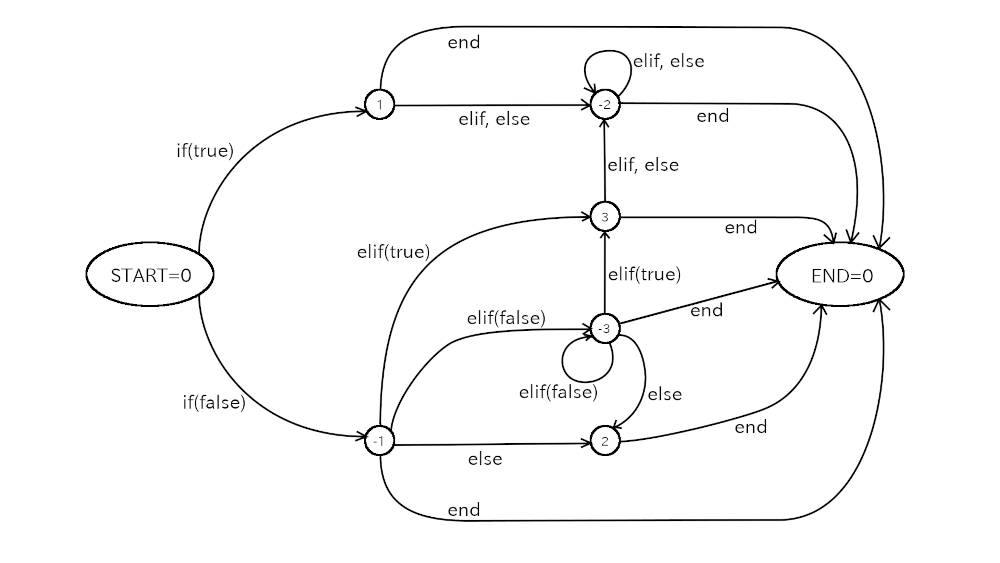
\includegraphics[width=15cm,height=8.4cm]{../image/state_diagram.png}
\caption{state diagram}
\end{figure}

\subsubsection{@@@table}\label{table}

This type of @@@ command starts with a line begins with ``@@@table''.
The contents of this command is a table of the GFM or pandoc's markdown.
The command makes a table easy to read. For example, a text file
\texttt{sample.md} has a table like this:

\begin{verbatim}
Price list

@@@table
|item|price|
|:---:|:---:|
|mouse|$10|
|PC|$500|
@@@
\end{verbatim}

The command changes this into:

\begin{verbatim}
Price list

|item |price|
|:---:|:---:|
|mouse| $10 |
| PC  |$500 |
\end{verbatim}

This command just changes the appearance of the table. There's no
influence on html/latex files that is converted from the markdown.
Notice that the command supports only the above type of markdown table
format.

A script \texttt{mktbl.rb} supports this command. If you run the script
like this:

\begin{verbatim}
$ ruby mktbl.rb sample.md
\end{verbatim}

Then, the tables in `sample.md' will be arranged. The script also makes
a backup file \texttt{sample.md.bak}.

The task of the script seems easy, but the program is not so simple. The
script \texttt{mktbl.rb} uses a library \texttt{lib/lib\_src2md.rb}

@@@commands are effective in the whole text. This means you can't stop
the @@@commands. But sometimes you want to show the commands literally
like this document. One solution is to add four blanks at the top of the
line. Then @@@commands are not effective because @@@commands must be at
the top of the line.

\subsection{Conversion}\label{conversion}

The @@@ commands are carried out by a method \texttt{src2md}, which is
in the file \texttt{lib/lib\_src2md.rb}. This method converts
\texttt{.src.md} file into \texttt{.md} file. In addition, some other
conversions are made by \texttt{src2md} method.

\begin{itemize}
\tightlist
\item
  Relative links are changed according to the change of the base
  directory.
\item
  Size option in an image link is removed when the destination is GFM or
  html.
\item
  Relative link is removed except .src.md files when the destination is
  html.
\item
  Relative link is removed when the destination is latex.
\end{itemize}

The order of the conversions are:

\begin{enumerate}
\def\labelenumi{\arabic{enumi}.}
\tightlist
\item
  @@@if
\item
  @@@table
\item
  @@@include
\item
  @@@shell
\item
  others
\end{enumerate}

There is the \texttt{src2md.rb} file in the top directory of this
repository. It just invokes the method \texttt{src2md}. In the same way,
the method is called in the action in the \texttt{Rakefile}.

\subsection{Directory structure}\label{directory-structure}

There are seven directories under \texttt{gtk4\_tutorial} directory.
They are \texttt{gfm}, \texttt{docs}, \texttt{latex}, \texttt{src},
\texttt{image}, \texttt{test} and \texttt{lib}. Three directories
\texttt{gfm}, \texttt{docs} and \texttt{latex} are the destination
directories for GFM, html and latex files respectively. It is possible
that these three directories don't exist before the conversion.

\begin{itemize}
\tightlist
\item
  src: This directory contains .src.md files and C-related source files.
\item
  image: This directory contains image files like png or jpg.
\item
  gfm: \texttt{rake} converts .src.md files to GFM files and store them
  in this directory.
\item
  docs: \texttt{rake\ html} will convert .src.md files to html files and
  store them in this directory.
\item
  latex: \texttt{rake\ pdf} will convert .src.md files to latex files
  and store them in this directory. Finally it creates a pdf file in
  \texttt{latex} directory.
\item
  lib: This directory includes ruby library files.
\item
  test: This directory contains test files. The tests are carried out by
  typing \texttt{rake\ test} on the terminal.
\end{itemize}

\subsection{Src directory and the top
directory}\label{src-directory-and-the-top-directory}

Src directory contains .src.md files and C-related source files. The top
directory, which is gtk\_tutorial directory, contains \texttt{Rakefile},
\texttt{src2md.rb} and some other files. When \texttt{Readme.md} is
generated, it will be located at the top directory. \texttt{Readme.md}
has title, abstract, table of contents with links to GFM files.

Rakefile describes how to convert .src.md files into GFM, html and/or
pdf files. Rake carries out the conversion according to the
\texttt{Rakefile}.

\subsection{The name of files in src
directory}\label{the-name-of-files-in-src-directory}

Files in \texttt{src} directory are an abstract, sections of the
document and other .src.md files. An \texttt{abstract.src.md} contains
the abstract of this tutorial. Each section filename is ``sec'', number
of the section and ``.src.md'' suffix. For example, ``sec1.src.md'',
``sec5.src.md'' or ``sec12.src.md''. They are the files correspond to
the section 1, section 5 and section 12 respectively.

\subsection{C source file directory}\label{c-source-file-directory}

Most of .src.md files have \texttt{@@@include} commands and they include
C source files. Such C source files are located in the subdirectories of
\texttt{src} directory.

Those C files have been compiled and tested. When you compile source
files, some auxiliary files and a target file like \texttt{a.out} are
created. Or \texttt{\_build} directory is made when \texttt{meson} and
\texttt{ninja} is used when compiling. Those files are not tracked by
\texttt{git} because they are specified in \texttt{.gitignore}.

The name of the subdirectories should be independent of section names.
It is because of renumbering, which will be explained in the next
subsection.

\subsection{Renumbering}\label{renumbering}

Sometimes you might want to insert a new section. For example, you want
to insert it between section 4 and section 5. You can make a temporary
section 4.5, that is a rational number between 4 and 5. However, section
numbers are usually integer so section 4.5 must be changed to section 5.
And the numbers of the following sections must be increased by one.

This renumbering is done by the \texttt{renumber} method in the
\texttt{lib/lib\_renumber.rb} file.

\begin{itemize}
\tightlist
\item
  It changes file names.
\item
  If there are references (links) to sections in .src.md files, the
  section numbers will be automatically renumbered.
\end{itemize}

\subsection{Rakefile}\label{rakefile}

Rakefile is similar to Makefile but controlled by rake, which is a ruby
script. Rakefile in this tutorial has the following tasks.

\begin{itemize}
\tightlist
\item
  md: generate GFM markdown files. This is the default.
\item
  html: generate html files.
\item
  pdf: generate latex files and a pdf file, which is compiled by
  lualatex.
\item
  all: generate md, html and pdf files.
\item
  clean: delete latex intermediate files.
\item
  clobber: delete all the generated files.
\end{itemize}

Rake does renumbering before the tasks above.

\subsection{Generate GFM markdown
files}\label{generate-gfm-markdown-files}

Markdown files (GFM) are generated by rake.

\begin{verbatim}
$ rake
\end{verbatim}

This command generates \texttt{Readme.md} with
\texttt{src/abstract.src.md} and titles of each \texttt{.src.md} file.
At the same time, it converts each .src.md file into a GFM file under
the \texttt{gfm} directory. Navigation lines are added at the top and
bottom of each markdown section file.

You can describe width and height of images in .src.md files. For
example,

\begin{verbatim}
![sample image](../image/sample_image.png){width=10cm height=6cm}
\end{verbatim}

The size between left brace and right brace is used in latex file and it
is not fit to GFM syntax. So the size will be removed in the conversion.

If a .src.md file has relative URL links, they will be changed by
conversion. Because .src.md files are located under the \texttt{src}
directory and GFM files are located under the \texttt{gfm} directory.
That means the base directory of the relative link are different. For
example, \texttt{{[}src/sample.c{]}(sample.c)} is translated to
\texttt{{[}src/sample.c{]}(../src/sample.c)}.

If a link points another .src.md file, then the target filename will be
changed to .md file. For example, \texttt{{[}Section\ 5{]}(sec5.src.md)}
is translated to \texttt{{[}Section\ 5{]}(sec5.md)}.

If you want to clean the directory, that means remove all the generated
markdown files, type \texttt{rake\ clobber}.

\begin{verbatim}
$ rake clobber
\end{verbatim}

Sometimes this is necessary before generating GFM files.

\begin{verbatim}
$ rake clobber
$ rake
\end{verbatim}

For example, if you append a new section and other files are still the
same as before, \texttt{rake\ clobber} is necessary. Because the
navigation of the previous section of the newly added section needs to
be updated. If you don't do \texttt{rake\ clobber}, then it won't be
updated because the the timestamp of .md file in gfm is newer than the
one of .src.md file. In this case, using \texttt{touch} to the previous
section .src.md also works to update the file.

If you see the GitHub repository (ToshioCP/Gtk4-tutorial),
\texttt{Readme.md} is shown below the code. And \texttt{Readme.md}
includes links to each markdown files. The repository not only stores
source files but also shows the whole tutorial.

\subsection{Generate html files}\label{generate-html-files}

Src.md files can be translated to html files. You need pandoc to do
this. Most linux distribution has pandoc package. Refer to your
distribution document to install.

Type \texttt{rake\ html} to generate html files.

\begin{verbatim}
$ rake html
\end{verbatim}

First, it generates pandoc's markdown files under \texttt{docs}
directory. Then, pandoc converts them to html files. The width and
height of image files are removed. Links to .src.md files will be
converted like this.

\begin{verbatim}
[Section 5](sec5.src.md) => [Section 5](sec5.html)
\end{verbatim}

Image files are copied to \texttt{docs/image} direcotiry and links to
them will be converted like this:

\begin{verbatim}
[sample.png](../image/sample.png) => [sample.png](image/sample.png)
\end{verbatim}

Other relative links will be removed.

\texttt{index.html} is the top html file. If you want to clean html
files, type \texttt{rake\ clobber} or \texttt{cleanhtml}.

\begin{verbatim}
$ rake clobber
\end{verbatim}

Every html file has a header
(\texttt{\textless{}head\textgreater{}\ -\/-\ \textless{}/head\textgreater{}}).
It is created by pandoc with `-s' option. You can customize the output
with your own template file for pandoc. Rake uses
\texttt{lib/lib\_mk\_html\_template.rb} to create its own template. The
template inserts bootstrap CSS and Javascript through \texttt{jsDelivr}.

The \texttt{docs} directory contains all the necessary html files. They
are used in the \href{https://ToshioCP.github.io/Gtk4-tutorial}{GitHub
pages} of this repository.

So if you want to publish this tutorial on your own web site, just
upload the files in the \texttt{docs} directory to your site.

\subsection{Generate a pdf file}\label{generate-a-pdf-file}

You need pandoc to convert markdown files into latex source files.

Type \texttt{rake\ pdf} to generate latex files and finally make a pdf
file.

\begin{verbatim}
$ rake pdf
\end{verbatim}

First, it generates pandoc's markdown files under \texttt{latex}
directory. Then, pandoc converts them into latex files. Links to files
or directories are removed because latex doesn't support them. However,
links to full URL and image files are kept. Image size is set with the
size between the left brace and right brace.

\begin{verbatim}
![sample image](../image/sample_image.png){width=10cm height=6cm}
\end{verbatim}

You need to specify appropriate width and height. It is almost
\texttt{0.015\ x\ pixels} cm. For example, if the width of an image is
400 pixels, the width in a latex file will be almost 6cm.

A file \texttt{main.tex} is the root file of all the generated latex
files. It has \texttt{\textbackslash{}input} commands, which inserts
each section file, between \texttt{\textbackslash{}begin\{document\}}
and \texttt{\textbackslash{}end\{document\}}. It also has
\texttt{\textbackslash{}input}, which inserts \texttt{helper.tex}, in
the preamble. Two files \texttt{main.tex} and \texttt{helper.tex} are
created by \texttt{lib/lib\_gen\_main\_tex.rb}. It has a sample markdown
code and converts it witn \texttt{pandoc\ -s}. Then, it extracts the
preamble in the generated file and puts it into \texttt{helper.tex}. You
can customize \texttt{helper.tex} by modifying
\texttt{lib/lib\_gen\_main\_tex.rb}.

Finally, lualatex compiles the \texttt{main.tex} into a pdf file.

If you want to clean \texttt{latex} directory, type
\texttt{rake\ clobber} or \texttt{rake\ cleanlatex}

\begin{verbatim}
$ rake clobber
\end{verbatim}

This removes all the latex source files and a pdf file.
